\documentclass{report}

\usepackage[headings]{fullpage}
\usepackage{scribe}

% Packages
\usepackage{amsfonts}
\usepackage{amsmath}
\usepackage{amsthm}
%\usepackage[letterpaper,margin=1in]{geometry}
\usepackage{epsfig}
\usepackage{color}
\usepackage{array}
\usepackage{pstricks}
\usepackage{pst-plot}
%\usepackage{pstricks-add}
\usepackage{multirow}

\theoremstyle{plain}
\newtheorem{lemma}{Lemma}
\newtheorem{claim}[lemma]{Claim}
\newtheorem{theorem}[lemma]{Theorem}
\newtheorem{corollary}[lemma]{Corollary}
\newtheorem{prop}[lemma]{Property}
\newtheorem{fact}[lemma]{Fact}

\theoremstyle{definition}
\newtheorem{define}[lemma]{Definition}
\newtheorem{example}[lemma]{Example}

\newtheorem{problem}{Problem}

\newcommand{\E}{\mathbb{E}}
\newcommand{\R}{\mathbb{R}}
\newcommand{\bP}{\mathbb{P}}
\newcommand{\var}{\mbox{\rm var}}
\newcommand{\pr}{\mbox{\rm Pr}}

\def\X{{\cal X}}
\def\cost{{\mbox{\rm cost}}}
\def\U{{\cal U}}

\begin{document}

\course{CSE 103}
\coursetitle{Probability and statistics}
\semester{Fall 2011}
\lecturer{}
\scribe{}
\lecturenumber{7}
\lecturetopic{Hashing and document comparison}

\maketitle

\section{Hashing}

In many situations, such as a dictionary application, we need to store a vast 
collection of items in such a way that we can look up any item instantaneously. 
The way to do this is by {\it hashing}.

\subsection{The hashing framework}

Suppose you have a large collection of items $x_1, \ldots, x_n$ that you want 
to store (for instance, all English words), where these items are 
drawn from some set $\U$ (for instance, the set of all conceivable words). 
The requirements are:
\begin{enumerate}
\item The total storage space used should be $O(n)$.
\item Given a query $q \in \U$, it should be possible to {\it very rapidly}
determine whether $q$ is one of the stored items $x_i$.
\end{enumerate}

\subsection{A simple solution using randomization}

\begin{enumerate}
\item Pick a completely random function $h: \U \rightarrow \{1,2,\ldots, n\}$. 

This is the {\it hash function}. 

\item Create a table $T$ of size $n$, each of whose entries is a pointer to a 
linked list, initialized to null. 

\item Store each $x_i$ in the linked list at $T[h(x_i)]$.

We say $x_i$ {\it hashes to} location $h(x_i)$.

\item Given a query $q$, look through the linked list at $T[h(q)]$ to see if
it's there.
\end{enumerate}

Here's a picture of the data structure.

\begin{center}
%%\resizebox{2.25in}{!}{\input{figs/table.pstex_t}}
\end{center}

The storage used is $O(n)$. What about the query time?

\subsection{Average query time}

Suppose query $q$ is picked at random, so that it is equally likely to hash to
any of the locations $1,2,\ldots, n$. What is the expected query time?
\begin{eqnarray*}
\mbox{Expected query time}
& =& 
\sum_{i=1}^n \pr(\mbox{$q$ hashes to location $i$}) \cdot \mbox{(length of list at $T[i]$)} \\
& =&
\frac{1}{n} \sum_i  \mbox{(length of list at $T[i]$)} \\ 
& = & 
\frac{1}{n} \cdot n \ = \ 1
\end{eqnarray*}
So the average query time is constant!

\subsection{Worst case query time, and a balls-in-bins problem}
\renewcommand{\log}{\mbox{log}_2}

What is the worst case query time; that is, what is the length of the longest linked list
in $T$? Equivalently, when you throw $n$ balls in $n$ bins, what is the size of the 
largest bin? We'll see that with very high probability, no bin gets $\geq \log n$
balls.

For any bin $i$, let $E_i$ be the event that it gets $\geq \log n$ balls.
$$ \pr(E_i) \  \leq \ {n \choose \log n} \left( \frac{1}{n} \right)^{\log n} .$$
(Do you see why?) 

To upper bound this probability we use the inequality (see cheat sheet) that
\[
{n \choose k} \leq \left( \frac{ne}{k} \right)^k
\]
Applying this inequality we get:
\[
{n \choose \log n} \left( \frac{1}{n} \right)^{\log n} \leq 
\left( \frac{ne}{n \log n}  \right)^{\log n} =
\left( \frac{e}{\log n}  \right)^{\log n} =
\frac{n^{\log e}}{(\log n)^{\log n}} \leq \frac{1}{n^2}
\]
Where the last inequality can be shown by moving the $n$ from the left
to the right and taking $1/x$ and then log of both sides:
\[
(\log n)(\log \log n) \geq (2+\log e) \log n
\]
Which holds when $n>2000$

Having shown that $\pr(E_i) \leq 1/n^2$, it follows that
$$ \pr(\mbox{some bin gets $\geq \log n$ balls})
\ = \ 
\pr(E_1 \cup E_2 \cup \cdots \cup E_n)
\ \leq \ 
\pr(E_1) + \cdots + \pr(E_n) 
\ \leq \ 
\frac{1}{n}.
$$
For instance, if you throw a million balls into a million bins, then the chance that
there is a bin with $\geq 20$ balls is at most 1 in a million.

Getting back to hashing, this means that the worst case query time is (with high
probability) $O(\mbox{log} n)$.

\subsection{The power of two choices}

Here's a variant on the balls and bins setup. As usual, you have before you a 
row of $n$ bins, along with a collection of $n$ identical balls. But now, 
when throwing each ball, {\it you pick two bins at random and you put the
ball in whichever of them is less full}.

It turns out, using an analysis that is too complicated to get into here, that
under this small change, the maximum bin size will be just $O(\log \log n)$ 
instead of $O(\log n)$.

This inspires an alternative hashing scheme:

\begin{enumerate}
\item Pick {\it two} completely random functions $h_1, h_2: \U \rightarrow \{1,2,\ldots, n\}$. 

\item Create a table $T$ of size $n$, each of whose entries is a pointer to a 
linked list, initialized to null. 

\item For each $x_i$, store it in either the linked list at $T[h_1(x_i)]$ or $T[h_2(x_i)]$,
whichever is shorter.

\item Given a query $q$, look through {\it both} the linked list at $T[h_1(q)]$ and
at $T[h_2(q)]$ to see if it's there.
\end{enumerate}

The storage requirement is still $O(n)$, the average query time is still $O(1)$, but now
the worst case query time drops to $O(\log \log n)$.

\section{Information retrieval}

When you go to Google and enter a query, like
\begin{quote}
{\tt what are treatment options for pneumonia}
\end{quote}
or
\begin{quote}
{\tt new song by radiohead}
\end{quote}
you immediately get back a list of highly suitable pages. It's as if the search engine
were instantaneously able to look through the tens of billions of pages on the web and
find the relevant ones. How does it pull this off? The answer is, by a combination of
clever preprocessing, statistics, hashing, and clustering.

In fact, these basic techniques apply not just to web search but to any system for
{\it information retrieval}: answering unstructured queries about a large collection
of documents.

\subsection{Preprocessing}

There are at five crucial preprocessing steps for a search engine.
\begin{enumerate}
\item Give each webpage a {\it reliability score}.

Most of the ``information'' on the web is grossly unreliable: spam, ignorant ravings, unfounded conjectures, and idle gossip. But we'll see (a bit later in the course) that it is possible to assess the reliability or authoritativeness of individual webpages --- by analyzing the statistics of linkage patterns.

\item Ignore {\it near-duplicates} of webpages.

More on this very shortly.

\item Discover the set of {\it terms}.

A {\it term} is an individual word, or a sequence of words that should be considered together, such as {\tt Katy Perry} or {\tt Rage Against the Machine}. Terms can be discovered by analyzing co-occurrence patterns. If a sequence of $k$ words keeps occurring together, they should be designated a term.

\item Create the {\it postings list}.

This is a hash table in which each term is associated with a linked list of the pages containing it.

\begin{center}
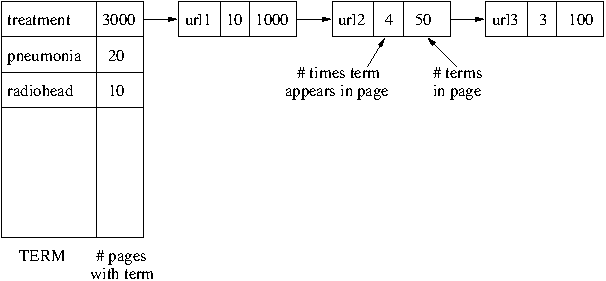
\includegraphics[width=5in]{figs/postings.pdf}
\end{center}

Each linked list is arranged in decreasing order of ``priority'' (some notion that takes into account reliability scores), and is usually truncated at a certain point.

\item Compute {\it term frequencies}.

How common is each term?

\end{enumerate}

\subsection{Answering a query}

The first step in answering a query is to order query terms by importance. The important terms are those that are uncommon. For instance, in
\begin{quote}
{\tt what are treatment options for pneumonia}
\end{quote}
the most important term is {\tt pneumonia}, since this is the least common. Next comes {\tt treatment}, and then {\tt options}. The remaining words are so common that they can be ignored.

The next step is to look at the postings list, and get all pages containing the important query term(s). Then, assign each a score based on:
\begin{itemize}
\item the reliability of that page
\item which of the important query terms it contains
\item the number of times each query term appears on that page, divided by the length of the page
\end{itemize}

This yields an ordered list of webpages, starting with the ``most relevant''. But the list will typically contain way too many pages. So they need to be clustered, and the user can then be presented with one representative page from each cluster, with the option to select ``more like this''.

For instance, pages about {\tt Rome} might be clustered into categories based on whether they refer to:
\begin{itemize}
\item Ancient Rome
\item Modern Rome
\item The TV series ``Rome''
\item and so on.
\end{itemize}

\section{Detecting near-duplicates}

Near-duplication is pervasive in the web: there are large numbers of distinct URLs which have exactly
the same content but differ only in unimportant details like headers and footers. The user of a search
engine would not be pleased if the answer to his query was a set of 10 near-identical pages! In order
to remove this redundancy, we need to define a notion of {\it similarity} between documents.

\subsection{The similarity between two documents}

For any document---call it $d$---let the set of all words in $d$ be denoted $C(d)$. For two documents 
$d$ and $d'$, we will measure their similarity by the function
$$ S(d,d') \ = \ \frac{|C(d) \cap C(d')|}{|C(d) \cup C(d')|} .$$
If the two documents are truly identical, $S(d,d') = 1$. If they are almost-identical, $S(d,d')$ will
be close to 1. And if they are completely different, with no words in common, then $S(d,d')$ will be
zero. We'll consider $d$ and $d'$ to be near-duplicates if $S(d,d')$ is sufficiently close to 1.

Now, imagine a search engine that is going through a list of documents or webpages, and wants to 
eliminate near-duplicates. Here's an algorithm it could use:
\begin{itemize}
\item ${\cal D} = \emptyset$ (set of documents, initially empty)
\item for each document $d$ that appears:
\begin{itemize}
\item if $S(d,d')$ is significantly smaller than 1 for all $d'$ in ${\cal D}$: add $d$ to ${\cal D}$
\end{itemize}
\end{itemize}
The final set of documents ${\cal D}$ will contain no near-duplicates. This is good, but the
algorithm is very slow. Suppose for the sake of simplicity that there are $n$ documents in total,
each of length $L$. Then computing the similarity between two documents takes $O(L)$ time, and
the algorithm is $O(n^2L)$. This quadratic dependence on $n$ is prohibitive in web-scale applications,
where $n$ could easily be in the billions or tens of billions.

To get a faster algorithm, we once again resort to hashing.

\subsection{An algorithm based on random permutations}

We will encode each document by a single number. Here's how.
\begin{itemize}
\item Pick any encoding of words as numbers: for instance, any word is in any case stored
as a binary number in the computer, and we can just use that number. Let $e(w)$ be the encoding
of word $w$. Suppose these encodings are in the range $1,\ldots, M$.
\item Let $\sigma$ be a {\it random permutation} of $(1,2,\ldots, M)$. Thus for each $i$, 
$\sigma(i)$ is a number in the range 1 to $M$, and all the $\sigma(i)$ are different.
\item Hash each document $d$ to the single number
$$ f(d) = \min \{\sigma(e(w)): w \in d\} .$$
That is, first think of all the words in the document as numbers, then apply the random 
permutation to each of these numbers (to get a different set of numbers), and finally pick
the smallest of these resulting numbers. It is important that the same permutation $\sigma$
is used for {\it all} the documents.
\end{itemize}

We will use the single number $f(d)$ in place of the entire document $d$! The rationale for doing 
this is captured in the following lemma, which says that near-duplicate documents are likely to
be hashed to the same value.
\begin{lemma}
Let $d,d'$ be any two documents. If $\sigma$ is a random permutation, then
$$ \pr(f(d) = f(d')) \ = \ S(d,d') .$$
\end{lemma}
\begin{proof}
For any word $w$, we will call $\sigma(e(w))$ its {\it value}.

Now, $f(d)$ and $f(d')$ will be equal if and only if the word in $d$ with the
smallest value is the same as the word in $d'$ with the smallest value. This is the same 
as saying that the smallest value among words in $d \cup d'$ lies in $d \cap d'$. The 
probability of this is exactly
$$ \frac{\mbox{\# words in $d \cap d'$}}{\mbox{\# words in $d \cup d'$}} \ = \ S(d,d').$$
Reason: $\sigma$ is a random permutation, so each word in $d \cup d'$ is equally likely to 
be the one with the smallest value.
\end{proof}

Here's the revised algorithm.
\begin{itemize}
\item Create a boolean array ${\tt seen}[1\ldots M]$, initialized to ${\tt false}$
\item ${\cal D} = \emptyset$ (set of documents, initially empty)
\item for each document $d$ that appears:
\begin{itemize}
\item if not ${\tt seen}[f(d)]$: add $d$ to ${\cal D}$ and set ${\tt seen}[f(d)] = {\tt true}$
\end{itemize}
\end{itemize}
This time, the running time is $O(nL)$, just linear in $n$.
\\

In practice, this algorithm is run not with the words in each document but with all 
sequences of $k$ words (called ``$k$-shingles''). For instance, the document
\begin{quote}
the quick brown fox jumped over the lazy dog
\end{quote}
has the following 3-shingles: {\tt the quick brown}, {\tt quick brown fox}, {\tt brown fox 
jumped}, {\tt fox jumped over}, {\tt jumped over the}, {\tt over the lazy}, {\tt the lazy dog}.

\end{document}



